\section{Probing the top quark vertices at the ILC}~\label{sec:top-elweak}

At higher energy, the study of $t\bar t$ pair production concentrates on the precise measurements of the couplings
of the $t$~quark to the $Z^0$~boson and the photon. 
 In contrast to the situation  at hadron colliders, the leading-order pair production process
$\ee\to t\bar t$ goes directly through the $t\bar{t} Z^0$ and 
$t\bar{t} \gamma$ vertices.  There is no concurrent QCD production 
of $\ttbar$ pairs, which increases greatly the potential for a clean measurement.
A commonly used expression to describe the  the current at the $t\bar{t} X$ vertex is~\cite{Juste:2006sv}

\begin{equation}\label{eq:gordon}
\Gamma_\mu^{ttX}(k^2,\,q,\,\bar{q}) = ie \left\{
  \gamma_\mu \, \left(  \widetilde{F}_{1V}^X(k^2)
                      + \gamma_5\widetilde{F}_{1A}^X(k^2) \right)
+ \frac{(q-\bar{q})_\mu}{2m_t}
    \left(  \widetilde{F}_{2V}^X(k^2)
          + \gamma_5\widetilde F_{2A}^X(k^2) \right)
\right\} .
\end{equation}
where $X = \gamma,Z$ and the  $\widetilde{F}$ are related to the usual
form factors $F_1$, $F_2$ by 
\begin{equation}
\label{eq:rel1}
\widetilde F^X_{1V} = -\left( F^X_{1V}+F^X_{2V} \right) \, , \qquad
\widetilde F^X_{2V}  =  F^X_{2V} \, , \qquad
\widetilde F^X_{1A} = -F^X_{1A} \, , \qquad
\widetilde F^X_{2A} =  -iF^X_{2A} \, .
%\label{eq:rel4}
\end{equation}
In the Standard Model the only form factors which are different 
from zero are $F_{1V}^\gamma(k^2),\,F_{1V}^{Z}(k^2)$ and $F_{1A}^{Z}(k^2)$.  The
quantities $F_{2V}^{\gamma,Z}(k^2)$ are the electric and weak magnetic dipole 
moment (EDM and MDM) form factors. The presence of the $\gamma/Z^0$ interference in electro-weak production gives sensitivity to the actual sign of the coupling constants. This is a distinct difference to the associated vector boson production at the LHC, which is only sensitive to their absolute values. 


In the following section, we will review the importance of measuring these couplings precisely.   Then we will describe studies of the experimental  capabilities of the ILC to perform these measurements. A great asset to test the chiral structure is the availability of polarized beams at the ILC. The studies presented in the following exploit this potential. For a full overview on the physics potential with polarised beams the reader is referred to~\cite{MoortgatPick:2005cw}.

\subsection{Top quark and new physics -  A brief motivation}

Neither the Standard Model of particle physics nor its super-symmetric extensions deliver an explanation for the striking mass hierarchy in the fermion sector. On the other hand, the mass hierarchy can be accommodated in models featuring extra dimensions, which are dual to models in which the $t$~quark and the Higgs Boson are composited objects. 
An example model with extra dimensions is that by Randall and Sundrum~\cite{Randall:1999ee}.  New physics will modify the electro-weak $\Zzero \ttbar$ vertex and modify the couplings $Q_L$ and $Q_R$ to the left- and right-chiral parts of the $\tpq$-quark wave-function. New physics may also entail the existence of a new $Z^{0'}$~boson or Kaluza-Klein excitations of the Standard Model $\Zzero$~boson. The modified vertex gives rise to different forward backward asymmetries $\afb$ than those predicted by the Standard Model. For this quantity a 3$\sigma$ discrepancy of the effective electro-weak mixing angle ${\rm sin}^{2}\theta_{eff}$ obtained in $b\bar{b}$ production at LEP has yet to be resolved~\cite{ALEPH:2005ab}. If this  effect is real, it is likely to be larger for the heavy $t$~quark.  
Please note that tensions with the Standard Model are also reported for the Tevatron results on $\afb$ in $\ttbar$ final states. 
The Standard Model prediction of the weak mixing angle is also challenged by the about  3$\sigma$ discrepancy observed in the
left right asymmetry $A_{LR}$ at the linear collider SLC, which featured linearly polarized electron beams. This measurement is the most precise measurement of $sin^{2}\theta_{eff}$ as of today. 
%If this  effect is real, it is likely to be larger for the heavy $t$ quark.

%Polarised beams will allow allow for the measurement of e.g. cross sections with different initial electron (positron) polarization.  This in turn permits also to measure the left-right asymmetry $\alr$, i.e. the change in cross-section for different beam polarisations. Here, too, a tension with Standard Model predictions has been observed at SLC~\cite{elwfits}.
 

% deviations have been measured for $\bottom$-quark at LEP~\cite{ALEPH:2005ab}.  The ILC will allow for polarised electron and positron beams. 
% for the $b$ quark at LEP result in 

%\subsection{Models with top and Higgs compositeness}

%There are several classes of models that seek to answer the question of 
%where the Higgs boson comes from and why it acquires a symmetry-breaking
%vacuum expectation value.  Among these is supersymmetry, which will have
%its own discussion in Section~7 of this report.  An alternative point of 
%view is that the Higgs boson is a composite state within a larger, strongly
%interacting theory at the TeV scale. Though the first models of this 
%type contained no light Higgs bosons, there are now many models that
%naturally contain a light Higgs boson very similar to
%the Higgs boson of the Standard Model coupling to new heavy particles at the
%TeV mass scale.  In Sections 2 and 4, we have described
%tests of models of this type at the ILC in the Higgs boson 
%and $W$ boson sectors.

%The top quark is the heaviest known particle that derives its mass 
%entirely from electro-weak symmetry breaking.  
%Due to its high mass the top quark couples to  the Higgs with a Yukawa 
%coupling of strength $\lambda_t \approx 1$.
%It is therefore likely that any composite structure
%of the Higgs boson must be reflected in composite structure or non-Standard
%interactions of the top quark.  While such interactions may exist, they
%may not be easy to find.   The coupling of the top quark to the gluon and
%the photon are constrained at $Q^2 = 0$ by requirements from exact QCD 
%and QED gauge invariance.   However, the low-energy $t\bar{t} Z$ vertex is
%much less constrained.   It is then likely that this is the crucial place 
%to look for deviations from the Standard Model induced by a strongly
%interacting Higgs sector.

%Models of composite Higgs bosons can be constructed in three ways that 
%seem at first sight to be distinctly different.  The Higgs bosons may be
%Goldstone bosons associated with strong-interaction symmetry breaking at
%the 10 TeV energy scale, as in Little Higgs models.   They may arise as 
%partners of gauge bosons in theories with an extra space dimension, as in 
%Gauge-Higgs Unification.  Or, they may arise in extra-dimensional theories
%as states confined to a lower-dimensional subspace or `brane'.   Randall
%and Sundrum constructed a model of the last type~\cite{Randall:1999ee}
% but also argued that 
%all three classes of models are related by strong coupling-weak coupling 
%duality~\cite{ArkaniHamed:2000ds}.   That is, it is possible to view the 
%extra-dimensional models as tools that allow weak coupling calculations of 
%effects that are intrinsically manifestations of strong coupling and 
%composite state dynamics.


%The Randall-Sundrum approach also includes a model explanation of the 
%hierarchy of Higgs-fermion Yukawa couplings.  This is one of the 
%most mysterious aspects of the Standard Model, reflected in the fact 
%that the top quark and the up quark have exactly the same quantum numbers
%but differ in mass by a factor of $10^5$.  The extra dimension 
%offers the possibility that the different flavors of fermion have 
%wavefunction of different shape in the full space, and therefore 
%different overlap with the wavefunction of the Higgs boson.  In general, 
%also, the right and left chiral components of each quark and lepton 
%may have wavefunctions with different dependence on the extra 
%dimensions.   It is a typical prediction of Randall-Sundrum theories
%that the chiral components of the top quark have wavefunctions in the 
%fifth dimension significantly different from those of the other quarks, 
%and significant different from one another, with the wavefunction of the
%right-handed top quark shifted significantly toward the low-energy 
%boundary of the space, called the `TeV brane', where the Higgs field is
%located.   These difference of the wavefunction are reflected directly 
%in couplings of the top quark to the $Z^0$ that are shifted from the 
%values predicted in the Standard Model, with larger shifts specifically
%for the right-handed top quark.  Figure~\ref{fig:cartoon-rs} collects a
%number of predictions of the fractional shift in the $t_L$ and $t_R$ 
%coupling to the $Z^0$ in a variety of models proposed in the literature.



%\begin{figure}
%\centering
%\includegraphics[width=0.7\columnwidth]{cartoon-rs.pdf}
%\caption{\sl Predictions of various groups~\cite{Djouadi:2006rk,Hosotani:2005nz,Cui:2010ds,Carena:2006bn}
% on deviations from Standard Model couplings of the t quark within 
%Randall-Sundrum Models. The cartoon is taken from~\cite{ild:bib:benchmark:doublet}.}
%\label{fig:cartoon-rs}
%\end{figure}

%Models with extra-dimensions may also be suited to explain the tensions
% observed at the Tevatron discussed in 
% Section~\ref{sec:asym-had}.   The top forward-backward asymmetry
%may, for example, be explained by a new color octet vector boson
% $G_{\mu}$, which couples weakly to light quarks but strongly to the
% $t$~quark.  This difference is required
% in order to suppress ordinary dijet production from the new colour-octet
% state. The difference in the coupling can be realised by the 
%arrangement of the $t$~quark wavefunction along the 
%extra-dimension~\cite{AguilarSaavedra:2012ma}.


\subsection{ILC measurements}

In the previous section, theories with extra dimensions and/or in which the 
$t$~quark and the Higgs boson are composite were briefly introduced. Compositeness is an
essential element of the physics of electro-weak symmetry breaking.
A key test of this idea would come from the measurement of the $t\bar
t Z$ couplings, where significant deviations from the predictions of
the Standard Model would be expected. The ILC provides an ideal environment to measure these couplings. 
At the ILC $\ttbar$ pairs would be copiously produced, several 100,000 events 
for an integrated luminosity of $500\,\invfb$.  The production is by
$s$-channel $\gamma$ and $\Zzero$~boson exchange, so the couplings to the $\Zzero$ enter the
cross section in order 1.  It is possible  to almost entirely eliminate the background from other Standard Model processes.  
%The ILC will
% allow for polarized electron and positron beams. This allows us
%to measure not only the total cross section for $t\bar t $ production 
%but also  the left-right asymmetry $\alr$, the change in 
%cross-section for different beam polarizations.  
%For the $b$ quark, The most precise measurements of $\alr$ at SLC and the 
%forward-backward asymmetry for the $b$ quark at LEP result in a 3 $\sigma$ discrepancy of 
%the effective electro-weak mixing angle $sin^{2}\theta_{eff}$ that has yet to be
%resolved~\cite{ALEPH:2005ab}.  If this  effect is real, it is likely to be larger for the heavy $t$ quark.

With the use of polarized beams, $t$ and $\bar t$ quarks oriented
toward different angular regions in the detector are enriched 
in left-handed or right-handed $t$~quark
polarization~\cite{Parke:1996pr}. 
This means that the experiments can independently access the 
couplings of left- and right-handed polarized quarks to the $\Zzero$~boson.
In principle, the measurement of the  cross section and forward-backward
asymmetry for two different polarization settings measures both the
photon and $\Zzero$~boson couplings of the $t$~quark for each handedness.
New probes of the $t$~quark  decay vertices are also available, although we expect that
these will already be highly constrained by the LHC measurements of
the $W$ polarization in $t$~quark decay.

%%%%%%%%%%%%%%%%%%%%%%%%%%%%%%%%%%%%%%%%%%%%%%%%%%% 
\begin{figure}
\centering
%\includegraphics[width=0.5\columnwidth, angle=270]{Top/AngDistTop.pdf}
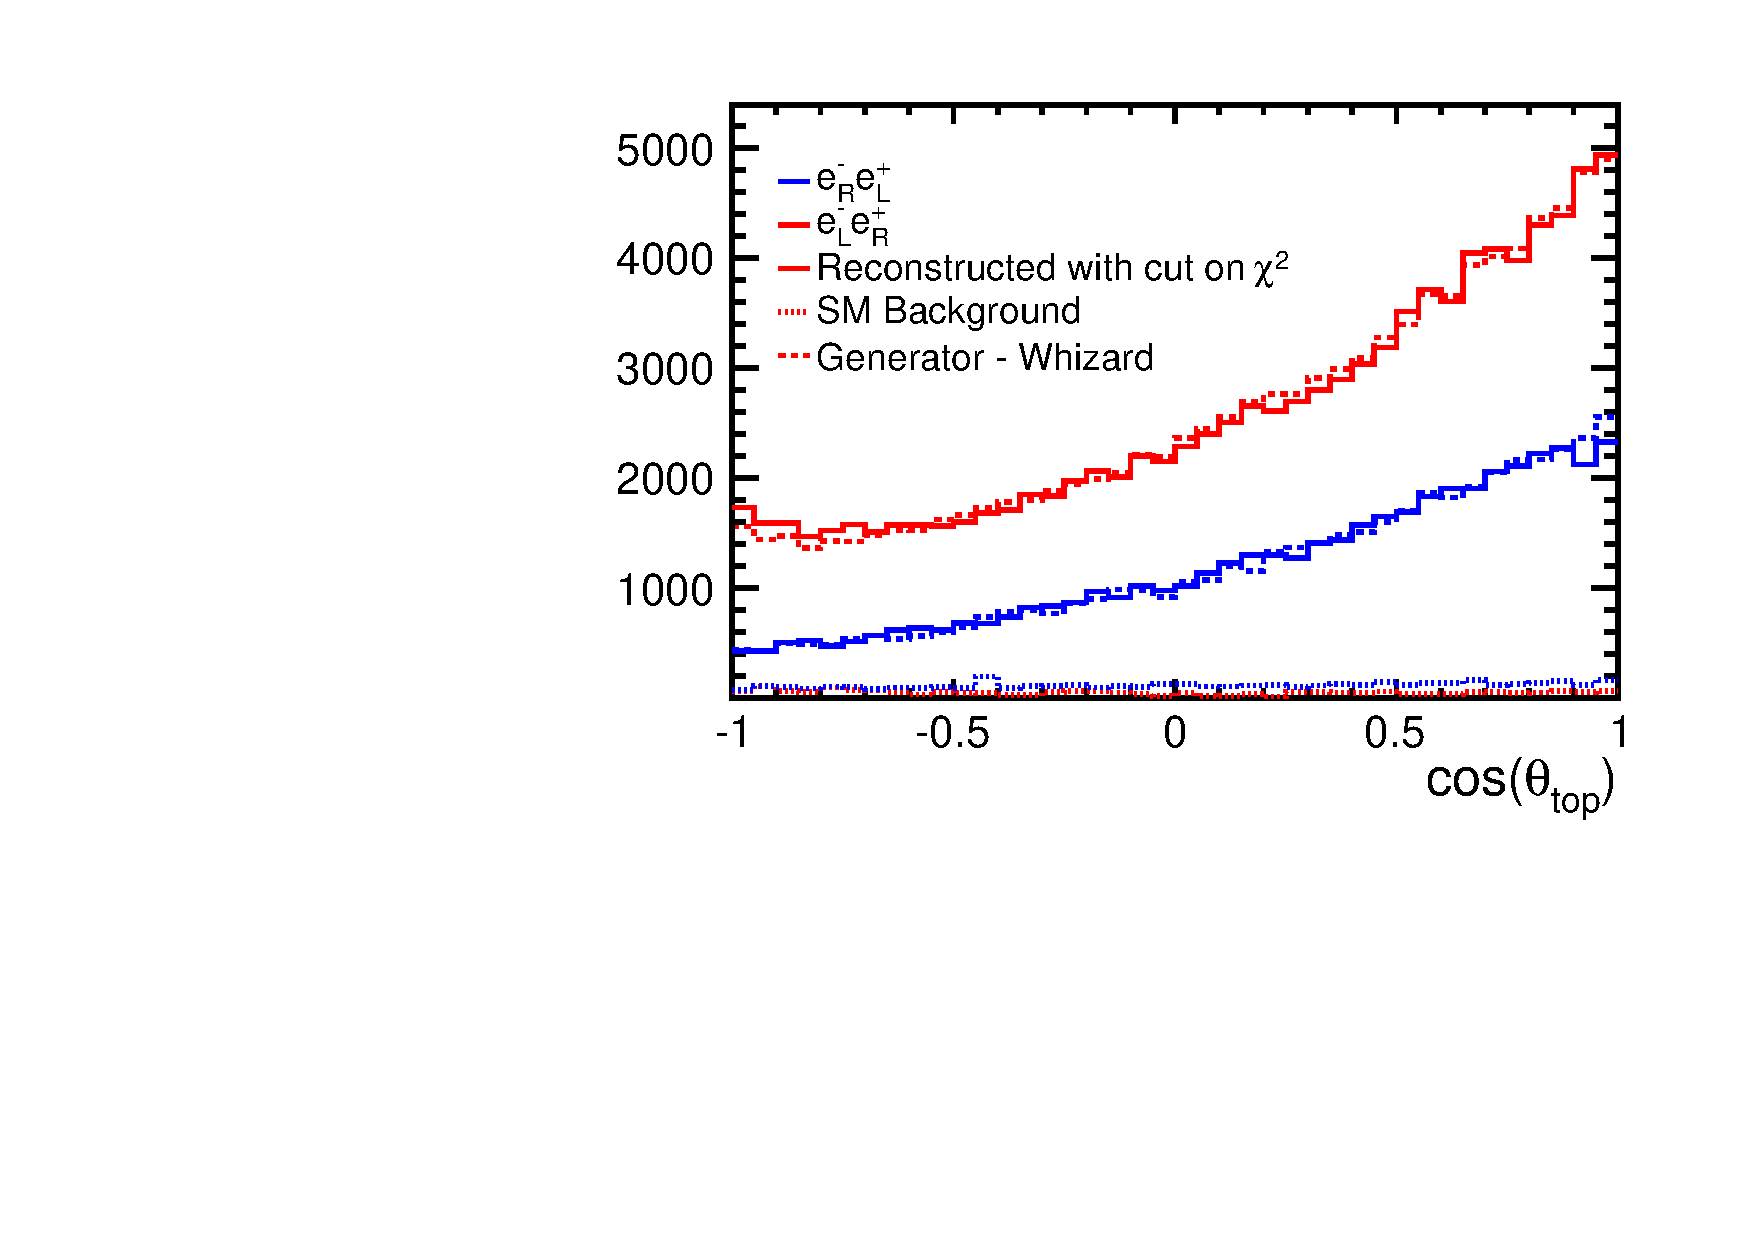
\includegraphics[width=0.7\columnwidth]{AFB_wbkg_chi2cut.pdf}
\caption{Reconstruction of the direction of the $t$ quark for two 
different beam polarization~\cite{Amjad:2013hca}. The population in the two different 
hemispheres w.r.t. the polar angle $\theta_{top}$ allows for the measurement of the forward-backward asymmetry $A_{FB}$. 
The residual Standard Model background is very small.}
%The plot shown is an update of one 
%presented in~\cite{top-lal}. Note that the figure does not include 
%background; however, it is known from the studies 
%in~\cite{ild:bib:benchmark:doublet} that the background is negligible.}
\label{fig:topangle}
\end{figure}
%%%%%%%%%%%%%%%%%%%%%%%%%%%%%%%%%%%%%%%%%%%%%%%%%%%%%%%%%%%%%%%%%%

Recent studies based on full simulation of ILC detectors for a center of mass
 energy of $\roots=500\,\GeV$ demonstrate that a precision on the 
determination of the couplings the left and the right chiral parts of 
the $t$~quark wave function to the $\Zzero$~boson of up to 1\% can be 
achieved~\cite{ild:bib:benchmark:doublet,Devetak:2010na,Doublet:2012wf}. The most recent example for such a study of semi-leptonic $\ttbar$ decays with full detector simulation is shown in Figure~\ref{fig:topangle}~\cite{Amjad:2013hca}.
The figure demonstrates the clean reconstruction of the $t$~quark direction, which allows for the precise determination of the 
forward-backward asymmetry, which is nearly free of Standard Model background.   It has to be noted however, that the final state gives rise to ambiguities in the correct association 
of the $b$~quarks to the $W$~bosons, see~\cite{Amjad:2013hca} for an explanation. These ambiguities can be nearly eliminated by requiring 
a high quality of the event reconstruction. The control of the ambiguities however requires an excellent detector performance and event reconstruction.
Another solution is the use of the vertex charge to separate the $t$ and $\bar t$~quark decays. It is shown in~\cite{Devetak:2010na} and confirmed in~\cite{bib:ilc-tdr-dbd} that the high efficiency of vertex tagging in the ILC detectors will make this strategy available. 
%The expected percent level independent measurements of the left- and right-handed top quark couplings will 
%clearly discriminate the models shown in Fig.~\ref{fig:cartoon-rs}.


Even more incisive measurements than presented using optimized 
observables are investigated in~\cite{Amjad:2013hca}. 
These observables are the $\ttbar$ pair production cross-section for left- 
and right-handed polarized beams and the fraction of right-handed ($t_R$) 
and left handed $t$~quarks ($t_L$).
Following a suggestion by~\cite{Berger:2012nw} for the Tevatron, the fraction 
of $t_L$ and $t_R$ in a given sample can be determined with the helicity 
asymmetry.  In the $t$~quark rest frame the distribution of the polar angle 
$\theta_{hel}$ of a decay lepton is 
\beq
\frac{1}{\Gamma} \frac{d\Gamma}{d\cthel} = \frac{1+ a_t \cthel}{2}  
\eeq{costhel}
where $a_t$ varies between $+1$ and $-1$ depending on the 
fraction of right-handed ($t_R$) and left handed $t$~quarks ($t_L$).
 The observable $\cthel$ can easily be measured at the ILC.  
This observable is much less sensitive to ambiguities in the 
event reconstruction than the forward backward asymmetry. The 
slope of the resulting linear distribution provides a very 
robust measure of the net polarization of a $t$~quark sample. The result of a full 
simulation study is shown in the top part of Fig.~\ref{fig:hel-coupl}.
 It is demonstrated that over a range in $\cthel$ the generated 
distribution is retained after event reconstruction. The 
reconstruction is nearly perfect for initial right handed electron beams. Remaining discrepancies in case of
 left handed electron beams can be explained by reconstruction 
inefficiencies for low energetic final state leptons. 

The introduced observables, i.e. $\afb$, cross sections and helicity asymmetry are used to disentangle the coupling of the $t$~quark to the photon and to the $\Zzero$.  
In the bottom part of  Fig.~\ref{fig:hel-coupl}, the precision on the form factors expected 
from the LHC and that from the ILC are compared with each other.
  
Numerical values for the expected accuracies at linear $e^+e^-$ colliders, ILC and earlier on TESLA~\cite{AguilarSaavedra:2001rg}, on seven $t$~quark form factors (due to QED gauge invariance the coupling $\widetilde F^\gamma_{1A}$ is fixed to 0), taken from the studies \cite{Abe:2001nq,AguilarSaavedra:2001rg,Amjad:2013hca},
are given in Tabs.~\ref{tab:tab1} and~\ref{tab:tab2}, along with comparisons to the expectations from 
the LHC experiments. Note in passing, that the replacement of TESLA results of Tab.~\ref{tab:tab2} by an ILC study is in preparation.  

From the comparison of the numbers it is justified to assume that the measurements at an electron positron collider lead to a spectacular improvement and thanks to the $\gamma/Z^0$ interference a $\epem$ collider can fix the sign the form factors. At the LHC the $t$~quark couples either to the photon or to the $Z^0$. In that case the cross section is proportional to e.g. $ (F^Z_{1V})^2 +  (F^Z_{1A})^2$. The precision expected at the LHC cannot exclude a sign flip of neither  $F^Z_{1V}$ nor of $F^Z_{1A}$. On the hand the LEP bounds can exclude a sign flip for $F^Z_{1A}$~\cite{Baur:2004uw}, which renders a much better precision for  $\widetilde F^Z_{1A}$ compared with $\widetilde F^Z_{1V}$. Clearly, the precisions that can be obtained at the LHC are to be revisited in the light of the real LHC data. A first result on associated production of vector boson and $\ttbar$ pairs is published in~\cite{Chatrchyan:2013qca}.


\begin{figure}
\centering
%\includegraphics[width=0.53\columnwidth]{Top/ThetaHelicity_Peskin.pdf}
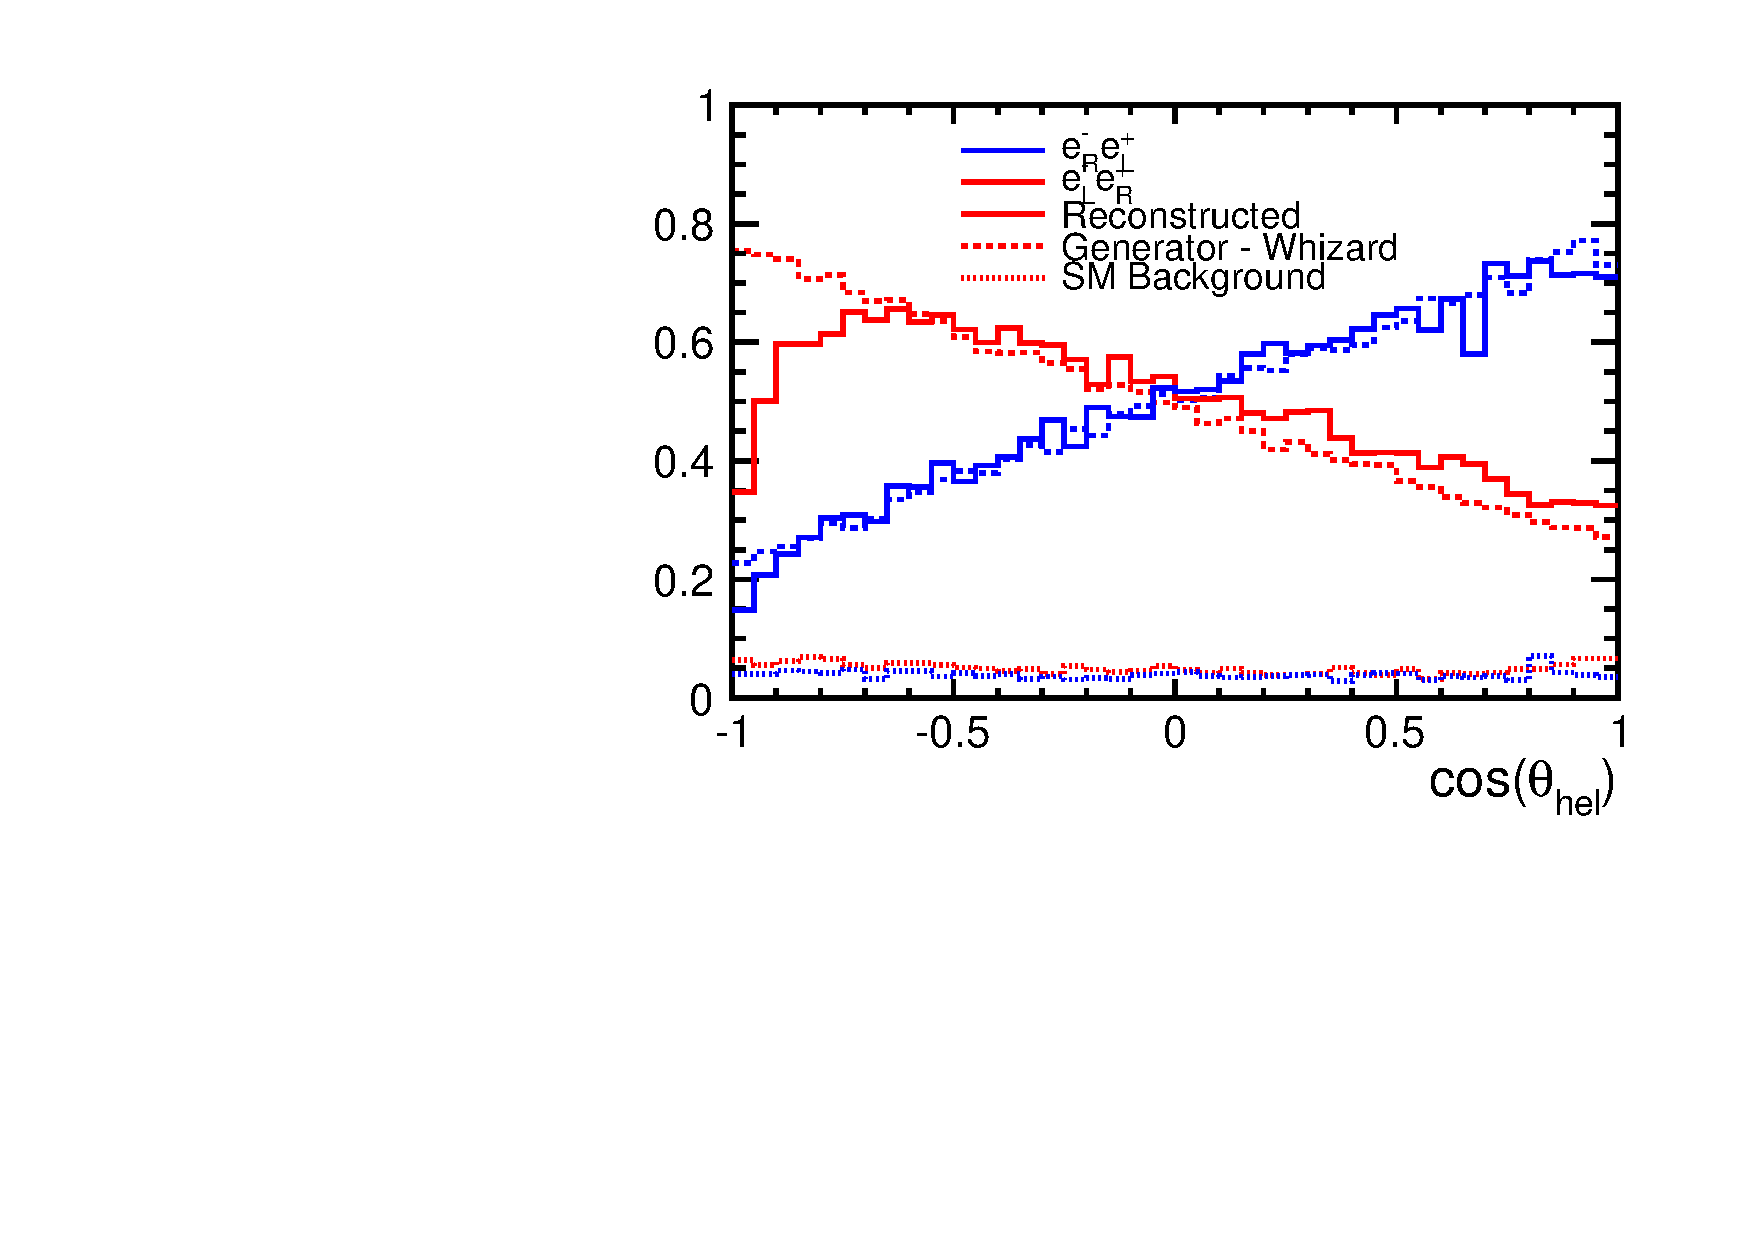
\includegraphics[width=0.63\columnwidth]{Helicity_wbkg.pdf}
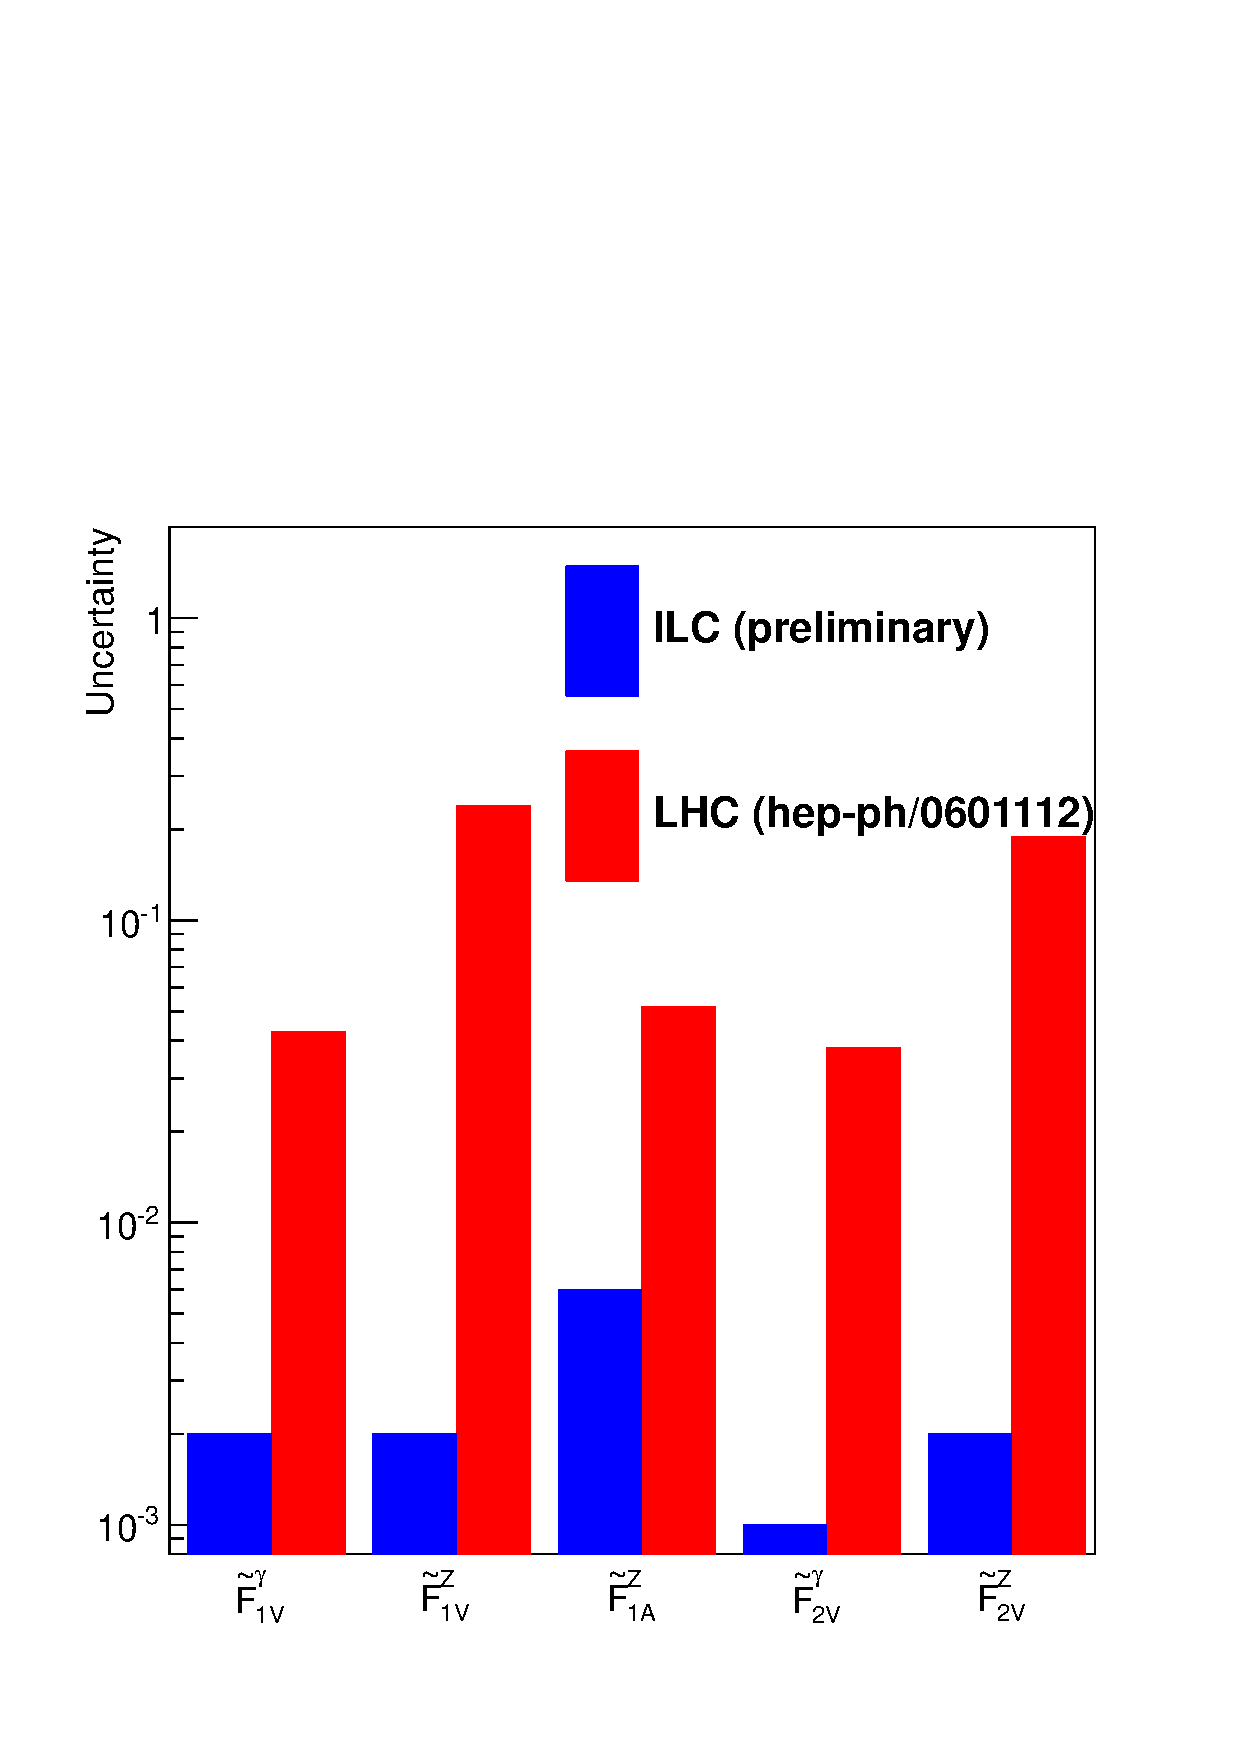
\includegraphics[width=0.63\columnwidth]{couplings.pdf}
\caption{
Top: Generated and reconstructed distribution of the helicity angle $\cthel$; 
Bottom: Comparison of precisions on $CP$ conserving form factors  
of the $t$~quark to $\gamma$ and $Z$, $\widetilde F^{\gamma,Z}_{1V,A}$,
expected at the LHC, taken from~\cite{Juste:2006sv}, and at the ILC. 
The LHC results assume an integrated luminosity of $\mathcal{L}=300~\invfb$.
The results for ILC~\cite{Amjad:2013hca} assume an integrated luminosity of $\mathcal{L}=500~\invfb$ at 
$\roots=500\,\GeV$ and a beam polarization  $P_{e^-} =\pm0.8,P_{e^+} = \mp0.3$.}
\label{fig:hel-coupl}
\end{figure}



\begin{table}[t]
\begin{center}
\begin{footnotesize}
%\begin{tabular}{ccc|ccc}
\begin{tabular}{|cccc|}
\hline
 Coupling & LHC~\protect\cite{Juste:2006sv}  & $e^+e^-$~\protect\cite{Abe:2001nq}&
           $e^+e^-$~\protect\cite{Amjad:2013hca}\\
 & $\mathcal{L}=300~\invfb$ & $P_{e^-}=\pm0.8$ & $\mathcal{L}=500~\invfb$,\, $P_{e^{-,+}} =\pm0.8,\mp0.3$
\\
\hline
$\Delta\widetilde F^\gamma_{1V}$ &
$\begin{matrix} +0.043 \\[-4pt] -0.041\end{matrix}$ &
$\begin{matrix} +0.047 \\[-4pt] -0.047 \end{matrix}$ ,
$\mathcal{L}=200~\invfb$&
%$\Delta\widetilde F^Z_{1V}$ &
%$\begin{matrix} +0.24 \\[-4pt]  -0.62\end{matrix}$ &
$\begin{matrix} +0.002 \\[-4pt] -0.002 \end{matrix}$
\\
%$\Delta\widetilde F^\gamma_{1A}$ &
%$\begin{matrix} +0.051 \\[-4pt] -0.048\end{matrix}$ &
%$\begin{matrix} +0.011 \\[-4pt] -0.011\end{matrix}$ ,
%    $\mathcal{L}=100~\invfb$ &
%$\Delta\widetilde F^Z_{1A}$ &
%$\begin{matrix} +0.052 \\[-4pt]  -0.060\end{matrix}$ &
%$\begin{matrix} +0.009 \\[-4pt] -0.009\end{matrix}$   \\
%$\Delta\widetilde F^\gamma_{2V}$ & $\begin{matrix} +0.038 \\[-4pt]
%-0.035\end{matrix}$ & $\begin{matrix} +0.038 \\[-4pt]
%-0.038\end{matrix}$ , 200~fb$^{-1}$  & $\Delta\widetilde F^Z_{2V}$ &
%$\begin{matrix} +0.27 \\[-4pt]
%-0.19\end{matrix}$ & $\begin{matrix} +0.009 \\[-4pt]
%-0.009\end{matrix}$ , 200~fb$^{-1}$
%\\
%$\Delta\widetilde F^\gamma_{2A}$ & $\begin{matrix} +0.16 \\[-4pt]
%-0.17\end{matrix}$ & $\begin{matrix} +0.014 \\[-4pt]
%-0.014\end{matrix}$ , 100~fb$^{-1}$   & $\Delta\widetilde F^Z_{2A}$ &
%$\begin{matrix} +0.28 \\[-4pt]
%-0.27\end{matrix}$ & $\begin{matrix} +0.052 \\[-4pt]
%-0.052\end{matrix}$ , 100~fb$^{-1}$
%\\
$\Delta\widetilde F^Z_{1V}$ &
$\begin{matrix} +0.24 \\[-4pt]  -0.62\end{matrix}$ &
$\begin{matrix} +0.012 \\[-4pt] -0.012\end{matrix}$ , $\mathcal{L}=200~\invfb$ &
%$\Delta\widetilde F^\gamma_{1V}$ &
%$\begin{matrix} +0.043 \\[-4pt] -0.041\end{matrix}$ &
$\begin{matrix} +0.002 \\[-4pt] -0.002\end{matrix}$
\\
$\Delta\widetilde F^Z_{1A}$ &
$\begin{matrix} +0.052 \\[-4pt]  -0.060\end{matrix}$ &
$\begin{matrix} +0.013 \\[-4pt] -0.013\end{matrix}$ , $\mathcal{L}=100~\invfb$ &
%$\Delta\widetilde F^\gamma_{1A}$ &
%$\begin{matrix} +0.051 \\[-4pt] -0.048\end{matrix}$ &
$\begin{matrix} +0.006 \\[-4pt] -0.006\end{matrix}$
\\
$\Delta\widetilde F^\gamma_{2V}$ &
$\begin{matrix} +0.038 \\[-4pt] -0.035\end{matrix}$ &
$\begin{matrix} +0.038 \\[-4pt] -0.038\end{matrix}$ , $\mathcal{L}=200~\invfb$&
%$\Delta\widetilde F^Z_{2V}$ &
%$\begin{matrix} +0.27 \\[-4pt]  -0.19\end{matrix}$ &
$\begin{matrix} +0.001 \\[-4pt] -0.001\end{matrix}$
\\
$\Delta\widetilde F^Z_{2V}$ &
$\begin{matrix} +0.27 \\[-4pt] -0.19\end{matrix}$ &
$\begin{matrix} +0.009 \\[-4pt] -0.009\end{matrix}$ , $\mathcal{L}=200~\invfb$  &
%$\Delta\widetilde F^Z_{2A}$ &
 $\begin{matrix} +0.002 \\[-4pt] -0.002\end{matrix}$
\\
%$\Delta\widetilde F^\gamma_{2V}$ &
%$\begin{matrix} +0.038 \\[-4pt] -0.035\end{matrix}$ &
%$\begin{matrix} +0.038 \\[-4pt] -0.038\end{matrix}$ , 200~fb$^{-1}$  &
%$\Delta\widetilde F^Z_{2V}$ &
%$\begin{matrix} +0.27 \\[-4pt]  -0.19\end{matrix}$ &
%$\begin{matrix} +0.009 \\[-4pt] -0.009\end{matrix}$ , $\mathcal{L}=200~\invfb$  &
%n.a.
%\\
%$\Delta\widetilde F^\gamma_{2A}$ &
%$\begin{matrix} +0.16 \\[-4pt] -0.17\end{matrix}$ &
%$\begin{matrix} +0.014 \\[-4pt] -0.014\end{matrix}$ , 100~fb$^{-1}$   &
%$\Delta\widetilde F^Z_{2A}$ &
%$\begin{matrix} +0.28 \\[-4pt]  -0.27\end{matrix}$ &
%$\begin{matrix} +0.052 \\[-4pt] -0.052\end{matrix}$ , $\mathcal{L}=100~\invfb$  &
%n.a.
%\\
\hline

\end{tabular}
\end{footnotesize}
\caption{Sensitivities achievable at $68.3\%$ CL for the
CP-conserving $t$~quark form factors $\widetilde F^X_{1V,A}$ and $\widetilde F^X_{2V}$ defined in \leqn{eq:gordon}, at LHC and at
the ILC.  The assumed luminosity samples and, for ILC, beam polarization,
 are indicated.
In the LHC studies and in the study
  \cite{Abe:2001nq}, only one form factor at a time is
allowed to deviate from its SM value.
In study~\cite{Amjad:2013hca} the form factors are allowed to vary independently. }
\label{tab:tab1}
\end{center}
\end{table}


\begin{table}[ht]
\begin{center}
\begin{footnotesize}
%\begin{tabular}{ccc|ccc}
\begin{tabular}{|ccc|}
\hline 
 Coupling & LHC~\protect\cite{Juste:2006sv}  &
           $e^+e^-$~\protect\cite{AguilarSaavedra:2001rg}\\
 & $\mathcal{L}=300~\invfb$ & 
$\mathcal{L}=300~\invfb$,\, $P_{e^{-,+}} =-0.8$
\\
\hline
%$\Delta\widetilde F_{2V}^{\gamma}$& $\begin{matrix} +0.038 \\[-4pt] -0.035\end{matrix}$ &  $\begin{matrix} +0.011 \\[-4pt] -0.011\end{matrix}$\\
%$\Delta\widetilde F_{2V}^{Z}$& $\begin{matrix} +0.27 \\[-4pt]  -0.19\end{matrix}$ &  $\begin{matrix} +0.011 \\[-4pt] -0.011\end{matrix}$\\
$\Delta {\mbox Re}\, \widetilde F_{2A}^{\gamma}$& $\begin{matrix} +0.17 \\[-4pt] -0.17\end{matrix}$ &$\begin{matrix} +0.007 \\[-4pt] -0.007\end{matrix}$   \\
$\Delta {\mbox Re}\, \widetilde F_{2A}^{Z}$& $\begin{matrix} +0.35 \\[-4pt] -0.35\end{matrix}$ &$\begin{matrix} +0.008 \\[-4pt] -0.008\end{matrix}$  \\
$\Delta {\mbox Im}\, \widetilde F_{2A}^{\gamma}$& $\begin{matrix} +0.17 \\[-4pt] -0.17\end{matrix}$  &$\begin{matrix} +0.008 \\[-4pt] -0.008\end{matrix}$  \\
$\Delta {\mbox Im}\, \widetilde F_{2A}^{Z}$& $\begin{matrix} +0.035 \\[-4pt] -0.035\end{matrix}$ & $\begin{matrix} +0.015 \\[-4pt] -0.015\end{matrix}$ \\
\hline
\end{tabular}
\end{footnotesize}
\caption{Sensitivities achievable at $68.3\%$ CL for the $t$~quark
CP-violating magnetic and electric dipole
form factors 
$\widetilde F^X_{2A}$ defined in \leqn{eq:gordon}, at the  LHC and at 
linear $e^+e^-$ colliders as published in the TESLA TDR.  The assumed luminosity samples and, for TESLA, the beam polarization,
 are indicated. In the LHC studies and in the TESLA studies, only one form factor at a time is 
allowed to deviate from its SM value. } 
\label{tab:tab2}
\end{center}
\end{table}

The expected high precision at a linear $\epem$ collider allow for a profound discussion of effects of new physics. The findings can be confronted with predictions in the framework of Randall-Sundrum models and/or compositeness models such as~\cite{Pomarol:2008bh,Djouadi:2006rk,Hosotani:2005nz,Cui:2010ds,Carena:2006bn,Grojean:2013qca} or Little Higgs models as e.g.~\cite{Berger:2005ht}. All these models entail deviations from the Standard Model values of the $t$~quark couplings to the $Z^0$ boson that will be measurable at the ILC. The interpretation of the results presented in Tables~\ref{tab:tab1} and~\ref{tab:tab2} in terms of the cited and maybe other models is in preparation and left for a future publication. {\em Comments and contributions from theory groups are highly welcome.}


%\begin{table}[ht!]
%\begin{center}
%\begin{tabular}{|l|c||cc|cc|} \hline
%begin{tabular}{|cc|}\hline
%Form factor  & $\sqrt{s}$  = 500\,GeV  \\
%\hline
%\hline
%&  $p$ = -- 0.8 \\
%\hline
% $F_{1V}^{\gamma}$ &\rule[-3mm]{0mm}{8mm} 1 
% &  &   &   &    \\
%$F_{1V}^{Z}$ &\rule[-3mm]{0mm}{8mm} 1 &  & 0.019 &  &     \\
%$F_{1A}^{Z}$ &\rule[-3mm]{0mm}{8mm} 1 &  & 0.016  &  &     \\
% $F_{1A}^{\gamma}$ &\rule[-3mm]{0mm}{8mm} 0
% &  &  &   &     \\
%$F_{2V}^{\gamma,Z}={(g-2)^{\gamma,Z}}_t$ &0.011  \\
%${\mbox Re}\, F_{2A}^{\gamma}$ &0.007   \\
%${\mbox Re}\, d_t^{\gamma}$ [10$^{-19}$ e cm] &\rule[-3mm]{0mm}{8mm} 0 & 20  & 4  & 8  &  2  \\
%${\mbox Re}\, F_{2A}^{Z}$ &0.008  \\
%${\mbox Re}\, d_t^{Z}$ [10$^{-19}$ e cm] &\rule[-3mm]{0mm}{8mm} 0 & 7  & 5  & 5  &  4  \\
%${\mbox Im}\, F_{2A}^{\gamma}$ &0.008  \\
%${\mbox Im}\, F_{2A}^{Z}$ & 0.015 \\
%\hline
%$F_{1R}^{W}$ &\rule[-3mm]{0mm}{8mm} 0 & 0.030 & 0.012 &   &     \\
%${\mbox Im} F_{2R}^{W}$ &\rule[-3mm]{0mm}{8mm} 0 & 0.025  &0.010 &  &     \\
%\hline
%\end{tabular}
%\caption[]{
%{1 s.d. statistical sensitivities to some (non) SM form factors
%in $t\bar t$ production \cite{top_18A,top_N24,top_rfrey} and in $t$ decay 
%to $Wb$ 
%\cite{top_18A,top_Bernreuther:1992be}. 
%The second column contains
%the respective SM value to lowest order, $p$ denotes the 
%polarisation of the electron beam.
%For the c.m. energy $\sqrt s$  = 500\GeV (800\GeV) an 
%integrated luminosity of 300 fb$^{-1}$ 
%(500 fb$^{-1}$) was used.
%$F_{1R}^{W}$ measures $(V+A)/(V-A)$.} \label{fig:top_topform} }
%\end{center}
%\end{table}


\subsubsection{Theory uncertainties on form factors - A brief outline}

The extraction of form factors requires precise predictions of the inclusive $\ttbar$ production rate and several differential distributions. 
As of today the QCD corrections are known to $N^3LO$ accuracy for the cross section and to $NNLO$ accuracy for $\afbt$. It is shown in~\cite{Amjad:2013hca} and references therein that the uncertainty on these corrections for the cross section are below 1\% with an even smaller scale uncertainty. Uncertainties for $\afbt$ yield about the same values.  

Electro-weak corrections are known to NLO accuracy. The correction for the cross section is about 5\% at $\roots=500\,\GeV$. The correction for $\afbt$ is between 10\% and 15\%~\cite{Fleischer:2003kk,Khiem:2012bp}. It is a major task for the future to estimate the size of the two-loop-correction and ultimately to calculate this contributions.

At this point it should also be noted that all of the studies on form factors are based on the WHIZARD event generator~\cite{Kilian:2007gr,Moretti:2001zz}.  This generator provides the final state in terms of six fermion events.
In particular the $\ttbar$ final state is indistinguishable from the final state of single $t$~quark production which give rise to interference terms. The contribution from single top events can be reduced by adequate kinematic cuts. Still, future studies will have to consider the residual contribution. 

%\subsubsection{An example: the Randall-Sundrum scenario}

%The sensitivity new physics can be paramerised by general dimension 
%six operators contributing to the $t\bar{t} \gamma $ and 
%$t\bar{t} Z $ vertex~\cite{AguilarSaavedra:2012vh}.  However, the potential of the ILC
%might be demonstrated more clearly by presenting a concrete example with
%one particular model.  In the original model of Randall and Sundrum~\cite{Randall:1999ee} there are additional
%massive gauge bosons in an assumed extra dimension. The model
%predicts increased couplings of the top quark, and perhaps 
%also the $b$ quark, to these Kaluza Klein particles. Following the analysis in ~\cite{Djouadi:2006rk,Djouadi:2009nb,Djouadi:2011aj}, one can 
%fix the parameters of the model so that these enhancements fit the
%two anomalies observed in the forward-backward asymmetry for $b$ quarks 
%$A_{FB,b}$ at LEP1 and for 
%top quarks  $A_{FB,t}$ at the Tevatron.  This gives a viable model of 
%top quark interactions associated with top and Higgs compositeness.
%Figure \ref{fig:hel-rs} shows the expected modifications of the 
%helicity angle distributions within this scenario.

 
%\begin{figure}
%\centering
%\includegraphics[width=0.7\columnwidth]{hel-rs.pdf}
%\caption{ 
%Distributions of the helicity angle  
%$\cthel$ expected from the Standard Model (thick lines) 
%and their modifications by the Randall-Sundrum framework 
%(thin lines) described in the text~\cite{Djouadi:2009nb}. The results are 
%shown for a beam polarization  $P_{e^-} =\pm 0.8,P_{e^+} = \mp 0.3$.}
%\label{fig:hel-rs}
%\end{figure}


%Both the slopes and total cross sections are deeply 
%modified in this scenario for the two polarizations. As explained 
%previously, these observables are directly measured at the ILC, and the 
%measurements allow one to fully disentangle the individual modifications
%of the $Z$ and photon couplings to top 
%quarks. It can also be shown 
%that by running at two energies, for instance 500\,GeV and 1\,TeV, 
%one can fully extract the
%parameters of the model, for instance, the Kaluza Klein boson masses, which 
%can be measured with about 1\% precision.  

%When the Kaluza Klein particles become very heavy, ILC at 500\,GeV can 
%observe deviations in  top 
%couplings at greater than 3 $\sigma$ 
%for masses which, depending on the details of the model,   
%typically range between 4 and 48\,TeV


%\subsubsection{Remarks on $(g-2)_t$}
%The determination of $\widetilde F^\gamma_{2V}$ gives access to anomalous magnetic moment $(g-2)_t$ in a rather simple way. For instance $\widetilde F^\gamma_{2V}=Q_t (g-2)_t /2$. $(g-2)_t$ receives Standard Model contributions from QED, QCD and EW~\cite{Grozin:2007fh}. One sees that this quantity will be measured to about 10\% accuracy. 

%What is known about $(g-2)_t$ ? In Ref.~\cite{Labun:2012fg} it said that that the limits on $g_t$ come from the 
%reaction $b \rightarrow s\gamma$  giving a very crude constraint : 
%\beq  
%                            -3.5 <  g_t < 3.6   
%\eeqn
%Ref.~\cite{Brodsky:1980zm} points out that $(g-2)_t$ is a very sensitive measurement for compositeness. For leptons one can 
%constrain compositeness at the 10000 TeV (~$10^{-18}\,\mathrm{cm}$) level. In other words e and $\mu$ are elementary 
%objects. This needs not be true for $t$~quarks. The expected precision on $(g-2)_t /2$ of 0.1\% is proportional to $m_t/M$ where $M$ 
%is the scale of compositeness. It follows hence that with the accuracy expected at the ILC the compositeness of the $t$~quark can be tested up to about 100\,TeV.
